\documentclass[12pt]{article}
\usepackage[margin=2.5cm]{geometry}
\usepackage{enumerate}
\usepackage{amsfonts}
\usepackage{amsmath}
\usepackage{fancyhdr}
\usepackage{amsmath}
\usepackage{amssymb}
\usepackage{amsthm}
\usepackage{mdframed}
\usepackage{graphicx}
\usepackage{subcaption}
\usepackage{adjustbox}
\usepackage{listings}
\usepackage{xcolor}
\usepackage{booktabs}
\usepackage[utf]{kotex}
\usepackage{hyperref}
\usepackage{accents}

\definecolor{codegreen}{rgb}{0,0.6,0}
\definecolor{codegray}{rgb}{0.5,0.5,0.5}
\definecolor{codepurple}{rgb}{0.58,0,0.82}
\definecolor{backcolour}{rgb}{0.95,0.95,0.92}

\lstdefinestyle{mystyle}{
    backgroundcolor=\color{backcolour},
    commentstyle=\color{codegreen},
    keywordstyle=\color{magenta},
    numberstyle=\tiny\color{codegray},
    stringstyle=\color{codepurple},
    basicstyle=\ttfamily\footnotesize,
    breakatwhitespace=false,
    breaklines=true,
    captionpos=b,
    keepspaces=true,
    numbers=left,
    numbersep=5pt,
    showspaces=false,
    showstringspaces=false,
    showtabs=false,
    tabsize=1
}

\lstset{style=mystyle}

\pagestyle{fancy}
\renewcommand{\headrulewidth}{0.4pt}
\lhead{CSC 343}
\rhead{Worksheet 4 Solution}

\begin{document}
\title{CSC343 Worksheet 4 Solution}
\maketitle

\bigskip
\begin{enumerate}[1.]
    \item
    \begin{enumerate}[a)]
        \item $[(1,0,1),(5,4,9),(1,0,1),(6,4,16),(7,9,16)]$
        \item $[(1,0),(3,3),(3,4),(4,3),(1,1),(4,3)]$
        \item $[(0,1),(0,1),(2,3),(2,4),(3,4)]$

        \bigskip

        \underline{\textbf{Notes:}}

        \bigskip

        \begin{itemize}
            \item $\tau_L(R)$ sorts tuples in order indicated by $L$.
            \begin{itemize}
                \item e.g.

                \bigskip

                $\tau_{C,B}(R)$ in $R(A,B,C)$ orders the tuples of $R$ by their
                values of $C$, and tuples with the same $C$-value are ordered by their
                $B$ value.
            \end{itemize}
        \end{itemize}

        \item $[(0,1),(0,2),(2,4),(2,5),(3,4),(3,4)]$
        \item $[(0,1),(2,4),(2,5),(3,4),(0,2)]$

        \bigskip

        \underline{\textbf{Notes:}}

        \bigskip

        \begin{itemize}
            \item $\delta(R)$ converts a bag into a set
            \begin{itemize}
                \item e.g.

                \bigskip

                Let $R = [(1,2),(3,4),(1,2),(1,2)]$

                \bigskip

                $\delta(R(A,B)) = [(1,2),(3,4)]$
            \end{itemize}
        \end{itemize}

        \item

        $[(0,2),(2,7),(3,4)]$

        \bigskip

        \underline{\textbf{Notes:}}

        \bigskip

        \begin{itemize}
            \item $\gamma_L(R)$ is an operator that groups a relation and/or aggregate
            some columns.

            \begin{itemize}
                \item L in $\gamma_L(R)$ is either
                \begin{enumerate}[1.]
                    \item \textbf{Grouping attribute} or an attribute by which R will be grouped.
                    \item \textbf{Aggregated attribute} or an attribute where an aggregation operator
                    is applied to.
                \end{enumerate}
            \end{itemize}

            \bigskip

            \underline{\textbf{Example:}}

            \bigskip

            $\gamma_{starName, MIN(year) \to minYear, COUNT(title) \to ctTitle}$(StarsIn)

            \bigskip

            \begin{center}
            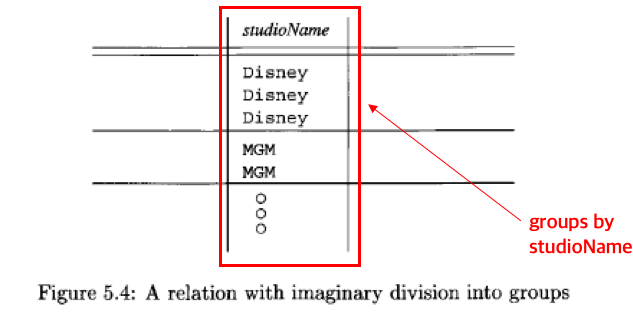
\includegraphics[width=0.7\linewidth]{images/worksheet_4_solution_1.png}
            \end{center}

        \end{itemize}

        \item $[(0, 1.5), (2, 4.5), (3,4)]$
        \item $[(0,1),(0,1),(2,3),(2,4),(3,4)]$
        \item $\gamma_{A, MAX(C)}([(2,3,4),(2,3,4)]) \to [(2,4)]$
        \item $[(0,1,\bot),(2,3,4), (2,3,4),(0,1,\bot),(2,4,\bot),(3,4,\bot)]$

        \bigskip

        \underline{\textbf{Notes:}}

        \bigskip

        \begin{itemize}
            \item $\accentset{\circ}{\bowtie}$ is an outerjoin operator
            \begin{itemize}
                \item $\accentset{\circ}{\bowtie}_L$ means Natural Left Outer Join
                \item $\accentset{\circ}{\bowtie}_R$ means Natural Right Outer Join
                \item $\accentset{\circ}{\bowtie}$ means Natural Full Outer Join
                \item $\bot$ means null
            \end{itemize}


            \item e.g. $U \accentset{\circ}{\bowtie} V$

            \bigskip

            \begin{center}
            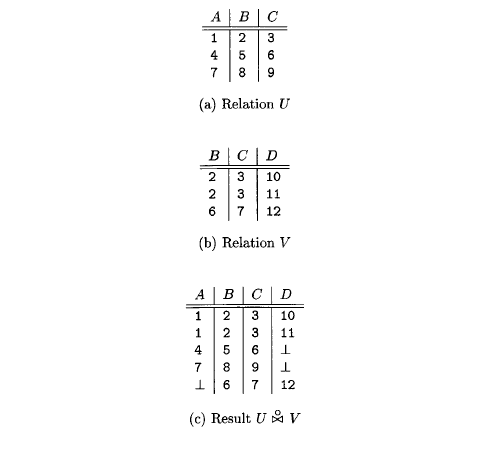
\includegraphics[width=0.7\linewidth]{images/worksheet_4_solution_2.png}
            \end{center}

        \end{itemize}

        \item $[(\bot,0,1),(\bot,2,4), (\bot,2,5),(2,3,4),(\bot,0,2),(2,3,4)]$
        \item $[(0,1,\bot),(2,3,4), (2,3,4),(0,1,\bot),(2,4,\bot),(3,4,\bot),\\
                (\bot,0,1),(\bot,2,4), (\bot,2,5),(2,3,4),(\bot,0,2),(2,3,4)]$
    \end{enumerate}
\end{enumerate}

\end{document}